% vim: ts=2:sw=2:tw=80:et
\thispagestyle{fancy}
\pagestyle{fancy}

\section{General Discussion}
Analog and digital output cards generally have the notion of changing the output
levels at times based upon some digital clock pulse.  As a very generic example,
a particular hardware device will have a list of output values that it is to
generate.  Each time that the rising edge (usually) of a clock pulse is
detected, the circuitry of the particular hardware device reads the next output
value and sets its actual output accordingly.

In some hardware, this notion of clock driven output is very explicit while for
other hardware, this notion is less explicit.  For Arbwave, regardless of the
function and/or capability of the hardware, each output device must have a
driving clock assigned explicitly to it.

\subsection{Sample/Update rates}
There will be two types of sample- or update-rates permissible.
\begin{itemize}
\item  Fixed update rates.
  An example of this would be a hardware card that updates a channel for every
  clock pulse and this clock pulse rate is fixed.  For hardware devices
  configured to operate with this type of update clock, the number of samples
  to update will automatically be calculated to the nearest clock pulse.
\item  Arbitrary timing update rates.
  Some hardware devices may be configured to use an arbitrary timing signal as
  the update clock.  An example of this would be when a channel from a
  Viewpoint DIO-64 card is configured to be used as a clock for other devices.
  For this type of configuration, the clock rate will automatically change
  such that the minimum number of clocks are emitted to support all
  channels/devices tied to the clock.  Clock pulses will designed to allow
  all voltage transitions as specified at their transition time within the
  maximum clock resolution possible (the internal clock rate of the DIO-64 for
  example).  In other words, a single waveform element may have a variable
  clock depending on whether other waveform channels similarly clocked need to
  have transitions in the mean time.
\end{itemize}


\begin{figure}[ht]
  \centerline{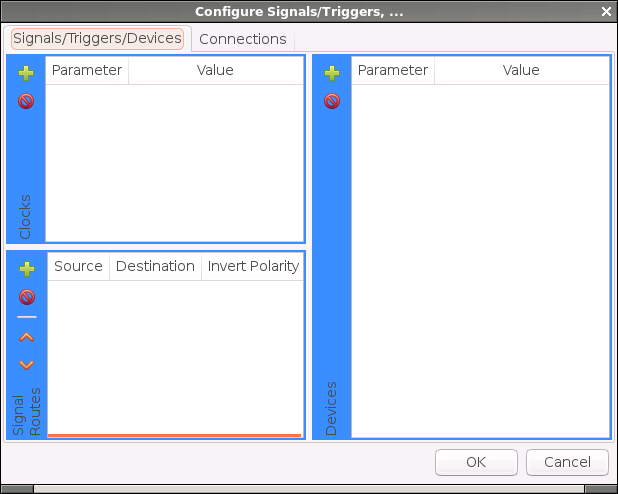
\includegraphics[width=.5\textwidth]{figures/empty}}
  \caption{Configuration window is empty upon startup}
  \label{fig:devcfg:empty}
\end{figure}



\section{Clocks}
In order to select a clock, you have to:
\begin{enumerate}
  \item define a clock in the clocks section (either by defining a
    counter--which does not work yet, or through an \signal{ao/SampleClock}, or something
    else)
  \item ensure that a route is defined from that clock to something that a
    particular device can connect to
    \begin{itemize}
      \item for instance, you can still define the \signal{ao/SampleClock} as your base
      clock
      \item then, in the routes section, define a route from
      \signal{$<$device-prefix$>$/ao/SampleClock} $\rightarrow$ \signal{TRIG/x}
    \end{itemize}
  \item Then, if Arbwave knows about how to make connections from the any of the
    defined clocks (either directly or through the information in the routes
    pane), you will be able to select one of the clocks that you defined in the
    clocks section.
\end{enumerate}

\begin{figure}[ht]
  \centerline{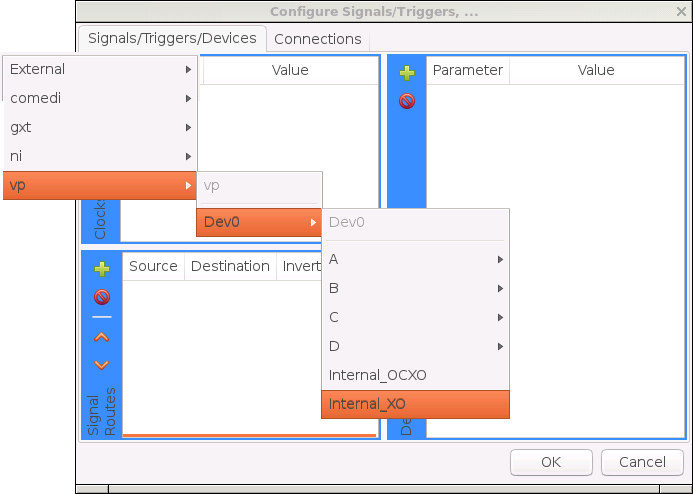
\includegraphics[width=.5\textwidth]{figures/add-clock-vp-XO}}
  \caption{Configuration window while adding a Viewpoint internal crystal
  oscillator for use as a clock}
  \label{fig:devcfg:add-clock-vp-XO}
\end{figure}

\begin{figure}[ht]
  \centerline{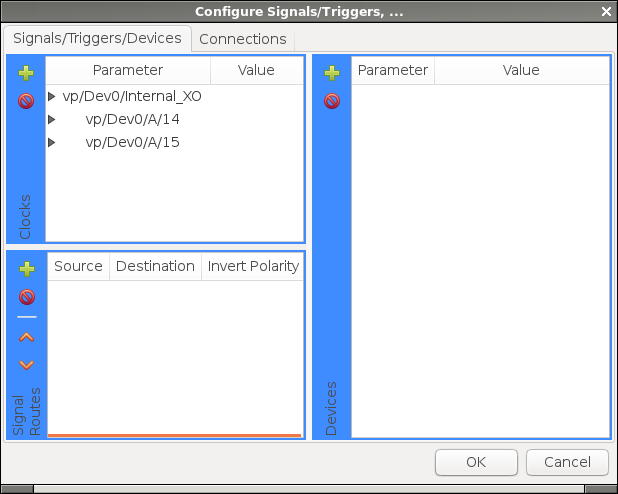
\includegraphics[width=.5\textwidth]{figures/clocks-added}}
  \caption{Configuration window after having added various possible clocks}
  \label{fig:devcfg:clocks-added}
\end{figure}


In other words, you would never really select any of the RTSI lines (aliased as
\signal{TRIG/0}--\signal{TRIG/7}) directly when you select a clock.
\textbf{But} you would probably need to define the routes properly so that
Arbwave knows it can use a given clock (and likely the actual RTSI line as the
physical connection).

For example, given that you have these devices:
\begin{itemize}
  \item \device{ni/Dev1/ao}  (the first PCI-6733 board)
  \item \device{ni/Dev2/ao}  (the second PCI-6733 board)
  \item \device{ni/Dev3/do}  (the PCI-6534 board)
\end{itemize}
Until we can get the counters working, you should be able to do:
\begin{enumerate}
  \item Define this clock and specify its rate as 1kHz for instance:\\
          \signal{ni/Dev1/ao/SampleClock}
          \begin{itemize}
            \item rate : 1000
          \end{itemize}
  \item Define a route from our clock to one of the RTSI lines:
         \signal{ni/Dev1/ao/SampleClock} $\rightarrow$ \signal{TRIG/0}
  \item Select \signal{ni/Dev1/ao/SampleClock} clock for all devices in the
    device pane.
\end{enumerate}


\section{Signal Routes}

\begin{figure}[ht]
  \centerline{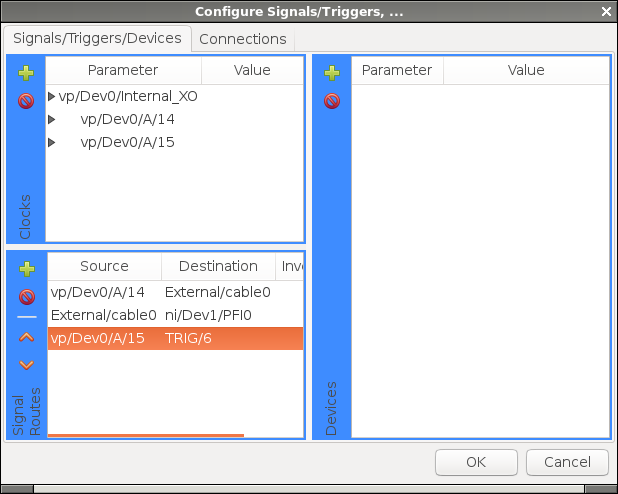
\includegraphics[width=.5\textwidth]{figures/routes-added}}
  \caption{Configuration window after defining signal routes for clocks}
  \label{fig:devcfg:routes-added}
\end{figure}


\section{Clock Sources for Devices}

\begin{figure}[ht]
  \centerline{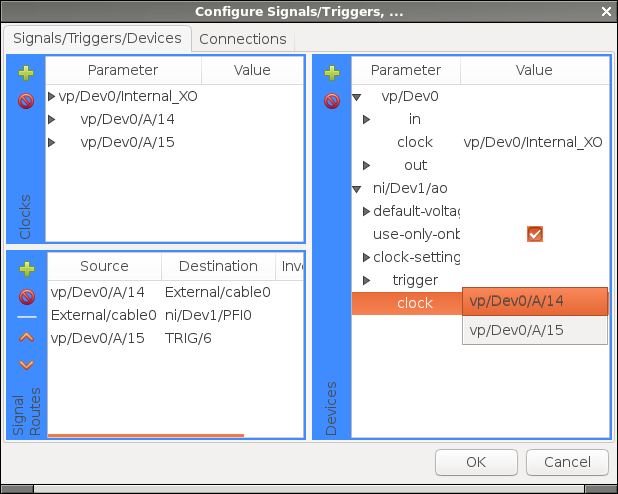
\includegraphics[width=.5\textwidth]{figures/devices-set-clocks}}
  \caption{Configuration window after assigning appropriate clocks to
  devices}
  \label{fig:devcfg:devices-set-clocks}
\end{figure}
